
\subsection{SDN}

%
% SDN
%
\begin{frame}\frametitle{SDN}

    \begin{itemize}
        \item Redes definidas por software (Software Defined Networking)
    \end{itemize}

    \begin{figure}[h]
        \centering
        
\includegraphics[scale=0.5]{images/sdn.jpg}
    \end{figure}
\end{frame}


%
% SDN
%
\begin{frame}\frametitle{SDN}

    \begin{itemize}
        \setlength{\itemsep}{1cm}
        \item Modelo que separa o plano de controle (decisões) do plano de 
            encaminhamento (comutação de pacotes). 
        \item Permite que pesquisadores façam experimentações e gerem 
            inovações na área de Redes de computadores 
            \citep{nick2008openflow}.
        \item Torna os elementos de comutação de uma rede programáveis
    \end{itemize}

\end{frame}


%
% Data plane
%
\begin{frame}\frametitle{Plano de dados}

    \begin{itemize}
    \item Encaminhamento de pacotes
    \item Comutação no \emph{hardware} do \emph{switch}
    \end{itemize}
        \begin{figure}[h]
        \centering
        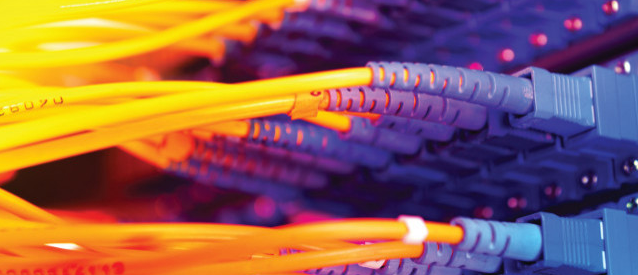
\includegraphics[scale=2.0]{images/data-plane.png}
    \end{figure}
\end{frame}


%
% Control plane
%
\begin{frame}\frametitle{Plano de controle}

    \begin{itemize}
    \item Decidir como encaminhar os pacotes
    \item Roteamento, políticas e visão topológica
    \end{itemize}
        \begin{figure}[h]
        \centering
        
\includegraphics[scale=0.5]{images/control-plane.png}
    \end{figure}
\end{frame}




%
% SDN
%
\begin{frame}\frametitle{SDN}

    \begin{itemize}
        \setlength{\itemsep}{1cm}
        \item SDN é apenas um modelo
        \item Um \emph{design} para construção e administração de redes
        \item A separação dos planos de controle e de dados torna o 
              funcionamento da rede mais flexível
    \end{itemize}
\end{frame}

%
% SDN
%
\begin{frame}\frametitle{Características}

    \begin{itemize}
        \setlength{\itemsep}{.5cm}
        \item Torna a rede programável
        \item Flexibilidade na administração da rede
        \item Controle logicamente centralizado
        \item Configurável via programação
        \item Padronização aberta 
    \end{itemize}
\end{frame}

